\documentclass[tikz,border=2pt]{standalone}
\usepackage{amsmath}
\usepackage{pgfplots}
\pgfplotsset{compat=1.18}
\usetikzlibrary{arrows.meta}
\begin{document}
% UDD with q_60 = 0.1: survival from 60 to 60+s is the straight line sp_60 = 1 - 0.1 s on [0,1].
% At s = 0.5 and 0.75 it is 0.95 and 0.925, so 0.25p_60.5 = 0.925/0.95 ~ 0.97368.
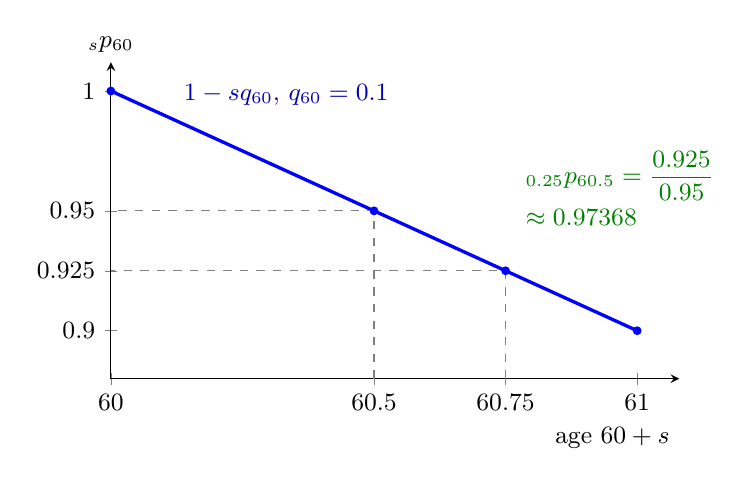
\begin{tikzpicture}[font=\small, >={Latex[length=2mm]}]
  \begin{axis}[
    axis lines=left, xmin=60, xmax=61.08, ymin=0.88, ymax=1.012,
    xtick={60,60.5,60.75,61}, xticklabels={$60$,$60.5$,$60.75$,$61$},
    ytick={0.9,0.925,0.95,1}, yticklabels={$0.9$,$0.925$,$0.95$,$1$},
    xlabel={age $60+s$}, ylabel={${}_sp_{60}$},
    xlabel style={at={(axis description cs:1,0)}, anchor=north east, yshift=-14pt},
    ylabel style={rotate=-90, at={(axis description cs:0,1)}, anchor=south},
    width=8.8cm, height=5.6cm, clip=false]
    \addplot[blue, very thick, domain=60:61] {1-0.1*(x-60)};
    \draw[gray, dashed] (axis cs:60.5,0.88) -- (axis cs:60.5,0.95) -- (axis cs:60,0.95);
    \draw[gray, dashed] (axis cs:60.75,0.88) -- (axis cs:60.75,0.925) -- (axis cs:60,0.925);
    \fill[blue] (axis cs:60.5,0.95) circle (1.6pt);
    \fill[blue] (axis cs:60.75,0.925) circle (1.6pt);
    \fill[blue] (axis cs:60,1) circle (1.6pt);
    \fill[blue] (axis cs:61,0.9) circle (1.6pt);
    \node[blue!70!black, anchor=south west] at (axis cs:60.12,0.99) {$1-sq_{60}$, $q_{60}=0.1$};
    \node[green!50!black, anchor=south west, align=left] at (axis cs:60.77,0.94)
      {${}_{0.25}p_{60.5}=\dfrac{0.925}{0.95}$\\[2pt]$\approx0.97368$};
  \end{axis}
\end{tikzpicture}
\end{document}
